% Options for packages loaded elsewhere
\PassOptionsToPackage{unicode}{hyperref}
\PassOptionsToPackage{hyphens}{url}
\PassOptionsToPackage{dvipsnames,svgnames,x11names}{xcolor}
%
\documentclass[
  letterpaper,
  DIV=11,
  numbers=noendperiod,
  oneside]{scrartcl}

\usepackage{amsmath,amssymb}
\usepackage{lmodern}
\usepackage{iftex}
\ifPDFTeX
  \usepackage[T1]{fontenc}
  \usepackage[utf8]{inputenc}
  \usepackage{textcomp} % provide euro and other symbols
\else % if luatex or xetex
  \usepackage{unicode-math}
  \defaultfontfeatures{Scale=MatchLowercase}
  \defaultfontfeatures[\rmfamily]{Ligatures=TeX,Scale=1}
\fi
% Use upquote if available, for straight quotes in verbatim environments
\IfFileExists{upquote.sty}{\usepackage{upquote}}{}
\IfFileExists{microtype.sty}{% use microtype if available
  \usepackage[]{microtype}
  \UseMicrotypeSet[protrusion]{basicmath} % disable protrusion for tt fonts
}{}
\makeatletter
\@ifundefined{KOMAClassName}{% if non-KOMA class
  \IfFileExists{parskip.sty}{%
    \usepackage{parskip}
  }{% else
    \setlength{\parindent}{0pt}
    \setlength{\parskip}{6pt plus 2pt minus 1pt}}
}{% if KOMA class
  \KOMAoptions{parskip=half}}
\makeatother
\usepackage{xcolor}
\usepackage[left=1in,marginparwidth=2.0666666666667in,textwidth=4.1333333333333in,marginparsep=0.3in]{geometry}
\setlength{\emergencystretch}{3em} % prevent overfull lines
\setcounter{secnumdepth}{-\maxdimen} % remove section numbering
% Make \paragraph and \subparagraph free-standing
\ifx\paragraph\undefined\else
  \let\oldparagraph\paragraph
  \renewcommand{\paragraph}[1]{\oldparagraph{#1}\mbox{}}
\fi
\ifx\subparagraph\undefined\else
  \let\oldsubparagraph\subparagraph
  \renewcommand{\subparagraph}[1]{\oldsubparagraph{#1}\mbox{}}
\fi

\usepackage{color}
\usepackage{fancyvrb}
\newcommand{\VerbBar}{|}
\newcommand{\VERB}{\Verb[commandchars=\\\{\}]}
\DefineVerbatimEnvironment{Highlighting}{Verbatim}{commandchars=\\\{\}}
% Add ',fontsize=\small' for more characters per line
\usepackage{framed}
\definecolor{shadecolor}{RGB}{241,243,245}
\newenvironment{Shaded}{\begin{snugshade}}{\end{snugshade}}
\newcommand{\AlertTok}[1]{\textcolor[rgb]{0.68,0.00,0.00}{#1}}
\newcommand{\AnnotationTok}[1]{\textcolor[rgb]{0.37,0.37,0.37}{#1}}
\newcommand{\AttributeTok}[1]{\textcolor[rgb]{0.40,0.45,0.13}{#1}}
\newcommand{\BaseNTok}[1]{\textcolor[rgb]{0.68,0.00,0.00}{#1}}
\newcommand{\BuiltInTok}[1]{\textcolor[rgb]{0.00,0.23,0.31}{#1}}
\newcommand{\CharTok}[1]{\textcolor[rgb]{0.13,0.47,0.30}{#1}}
\newcommand{\CommentTok}[1]{\textcolor[rgb]{0.37,0.37,0.37}{#1}}
\newcommand{\CommentVarTok}[1]{\textcolor[rgb]{0.37,0.37,0.37}{\textit{#1}}}
\newcommand{\ConstantTok}[1]{\textcolor[rgb]{0.56,0.35,0.01}{#1}}
\newcommand{\ControlFlowTok}[1]{\textcolor[rgb]{0.00,0.23,0.31}{#1}}
\newcommand{\DataTypeTok}[1]{\textcolor[rgb]{0.68,0.00,0.00}{#1}}
\newcommand{\DecValTok}[1]{\textcolor[rgb]{0.68,0.00,0.00}{#1}}
\newcommand{\DocumentationTok}[1]{\textcolor[rgb]{0.37,0.37,0.37}{\textit{#1}}}
\newcommand{\ErrorTok}[1]{\textcolor[rgb]{0.68,0.00,0.00}{#1}}
\newcommand{\ExtensionTok}[1]{\textcolor[rgb]{0.00,0.23,0.31}{#1}}
\newcommand{\FloatTok}[1]{\textcolor[rgb]{0.68,0.00,0.00}{#1}}
\newcommand{\FunctionTok}[1]{\textcolor[rgb]{0.28,0.35,0.67}{#1}}
\newcommand{\ImportTok}[1]{\textcolor[rgb]{0.00,0.46,0.62}{#1}}
\newcommand{\InformationTok}[1]{\textcolor[rgb]{0.37,0.37,0.37}{#1}}
\newcommand{\KeywordTok}[1]{\textcolor[rgb]{0.00,0.23,0.31}{#1}}
\newcommand{\NormalTok}[1]{\textcolor[rgb]{0.00,0.23,0.31}{#1}}
\newcommand{\OperatorTok}[1]{\textcolor[rgb]{0.37,0.37,0.37}{#1}}
\newcommand{\OtherTok}[1]{\textcolor[rgb]{0.00,0.23,0.31}{#1}}
\newcommand{\PreprocessorTok}[1]{\textcolor[rgb]{0.68,0.00,0.00}{#1}}
\newcommand{\RegionMarkerTok}[1]{\textcolor[rgb]{0.00,0.23,0.31}{#1}}
\newcommand{\SpecialCharTok}[1]{\textcolor[rgb]{0.37,0.37,0.37}{#1}}
\newcommand{\SpecialStringTok}[1]{\textcolor[rgb]{0.13,0.47,0.30}{#1}}
\newcommand{\StringTok}[1]{\textcolor[rgb]{0.13,0.47,0.30}{#1}}
\newcommand{\VariableTok}[1]{\textcolor[rgb]{0.07,0.07,0.07}{#1}}
\newcommand{\VerbatimStringTok}[1]{\textcolor[rgb]{0.13,0.47,0.30}{#1}}
\newcommand{\WarningTok}[1]{\textcolor[rgb]{0.37,0.37,0.37}{\textit{#1}}}

\providecommand{\tightlist}{%
  \setlength{\itemsep}{0pt}\setlength{\parskip}{0pt}}\usepackage{longtable,booktabs,array}
\usepackage{calc} % for calculating minipage widths
% Correct order of tables after \paragraph or \subparagraph
\usepackage{etoolbox}
\makeatletter
\patchcmd\longtable{\par}{\if@noskipsec\mbox{}\fi\par}{}{}
\makeatother
% Allow footnotes in longtable head/foot
\IfFileExists{footnotehyper.sty}{\usepackage{footnotehyper}}{\usepackage{footnote}}
\makesavenoteenv{longtable}
\usepackage{graphicx}
\makeatletter
\def\maxwidth{\ifdim\Gin@nat@width>\linewidth\linewidth\else\Gin@nat@width\fi}
\def\maxheight{\ifdim\Gin@nat@height>\textheight\textheight\else\Gin@nat@height\fi}
\makeatother
% Scale images if necessary, so that they will not overflow the page
% margins by default, and it is still possible to overwrite the defaults
% using explicit options in \includegraphics[width, height, ...]{}
\setkeys{Gin}{width=\maxwidth,height=\maxheight,keepaspectratio}
% Set default figure placement to htbp
\makeatletter
\def\fps@figure{htbp}
\makeatother

\KOMAoption{captions}{tableheading}
\makeatletter
\@ifpackageloaded{tcolorbox}{}{\usepackage[many]{tcolorbox}}
\@ifpackageloaded{fontawesome5}{}{\usepackage{fontawesome5}}
\definecolor{quarto-callout-color}{HTML}{909090}
\definecolor{quarto-callout-note-color}{HTML}{0758E5}
\definecolor{quarto-callout-important-color}{HTML}{CC1914}
\definecolor{quarto-callout-warning-color}{HTML}{EB9113}
\definecolor{quarto-callout-tip-color}{HTML}{00A047}
\definecolor{quarto-callout-caution-color}{HTML}{FC5300}
\definecolor{quarto-callout-color-frame}{HTML}{acacac}
\definecolor{quarto-callout-note-color-frame}{HTML}{4582ec}
\definecolor{quarto-callout-important-color-frame}{HTML}{d9534f}
\definecolor{quarto-callout-warning-color-frame}{HTML}{f0ad4e}
\definecolor{quarto-callout-tip-color-frame}{HTML}{02b875}
\definecolor{quarto-callout-caution-color-frame}{HTML}{fd7e14}
\makeatother
\makeatletter
\makeatother
\makeatletter
\makeatother
\makeatletter
\@ifpackageloaded{caption}{}{\usepackage{caption}}
\AtBeginDocument{%
\ifdefined\contentsname
  \renewcommand*\contentsname{Table of contents}
\else
  \newcommand\contentsname{Table of contents}
\fi
\ifdefined\listfigurename
  \renewcommand*\listfigurename{List of Figures}
\else
  \newcommand\listfigurename{List of Figures}
\fi
\ifdefined\listtablename
  \renewcommand*\listtablename{List of Tables}
\else
  \newcommand\listtablename{List of Tables}
\fi
\ifdefined\figurename
  \renewcommand*\figurename{Figure}
\else
  \newcommand\figurename{Figure}
\fi
\ifdefined\tablename
  \renewcommand*\tablename{Table}
\else
  \newcommand\tablename{Table}
\fi
}
\@ifpackageloaded{float}{}{\usepackage{float}}
\floatstyle{ruled}
\@ifundefined{c@chapter}{\newfloat{codelisting}{h}{lop}}{\newfloat{codelisting}{h}{lop}[chapter]}
\floatname{codelisting}{Listing}
\newcommand*\listoflistings{\listof{codelisting}{List of Listings}}
\makeatother
\makeatletter
\@ifpackageloaded{caption}{}{\usepackage{caption}}
\@ifpackageloaded{subcaption}{}{\usepackage{subcaption}}
\makeatother
\makeatletter
\@ifpackageloaded{tcolorbox}{}{\usepackage[many]{tcolorbox}}
\makeatother
\makeatletter
\@ifundefined{shadecolor}{\definecolor{shadecolor}{rgb}{.97, .97, .97}}
\makeatother
\makeatletter
\@ifpackageloaded{sidenotes}{}{\usepackage{sidenotes}}
\@ifpackageloaded{marginnote}{}{\usepackage{marginnote}}
\makeatother
\makeatletter
\makeatother
\ifLuaTeX
  \usepackage{selnolig}  % disable illegal ligatures
\fi
\IfFileExists{bookmark.sty}{\usepackage{bookmark}}{\usepackage{hyperref}}
\IfFileExists{xurl.sty}{\usepackage{xurl}}{} % add URL line breaks if available
\urlstyle{same} % disable monospaced font for URLs
\hypersetup{
  pdftitle={A straightforward strategy to get your Shiny app online, securely and continuously updated.},
  pdfauthor={Ronald (Ryy) Glenn Thomas},
  colorlinks=true,
  linkcolor={blue},
  filecolor={Maroon},
  citecolor={Blue},
  urlcolor={Blue},
  pdfcreator={LaTeX via pandoc}}

\title{A straightforward strategy to get your Shiny app online, securely
and continuously updated.}
\usepackage{etoolbox}
\makeatletter
\providecommand{\subtitle}[1]{% add subtitle to \maketitle
  \apptocmd{\@title}{\par {\large #1 \par}}{}{}
}
\makeatother
\subtitle{Github, Docker-compose, EC2 version}
\author{Ronald (Ryy) Glenn Thomas}
\date{}

\begin{document}
\maketitle
\ifdefined\Shaded\renewenvironment{Shaded}{\begin{tcolorbox}[frame hidden, sharp corners, borderline west={3pt}{0pt}{shadecolor}, boxrule=0pt, enhanced, interior hidden, breakable]}{\end{tcolorbox}}\fi

\renewcommand*\contentsname{Table of contents}
{
\hypersetup{linkcolor=}
\setcounter{tocdepth}{3}
\tableofcontents
}
\marginnote{\begin{footnotesize}

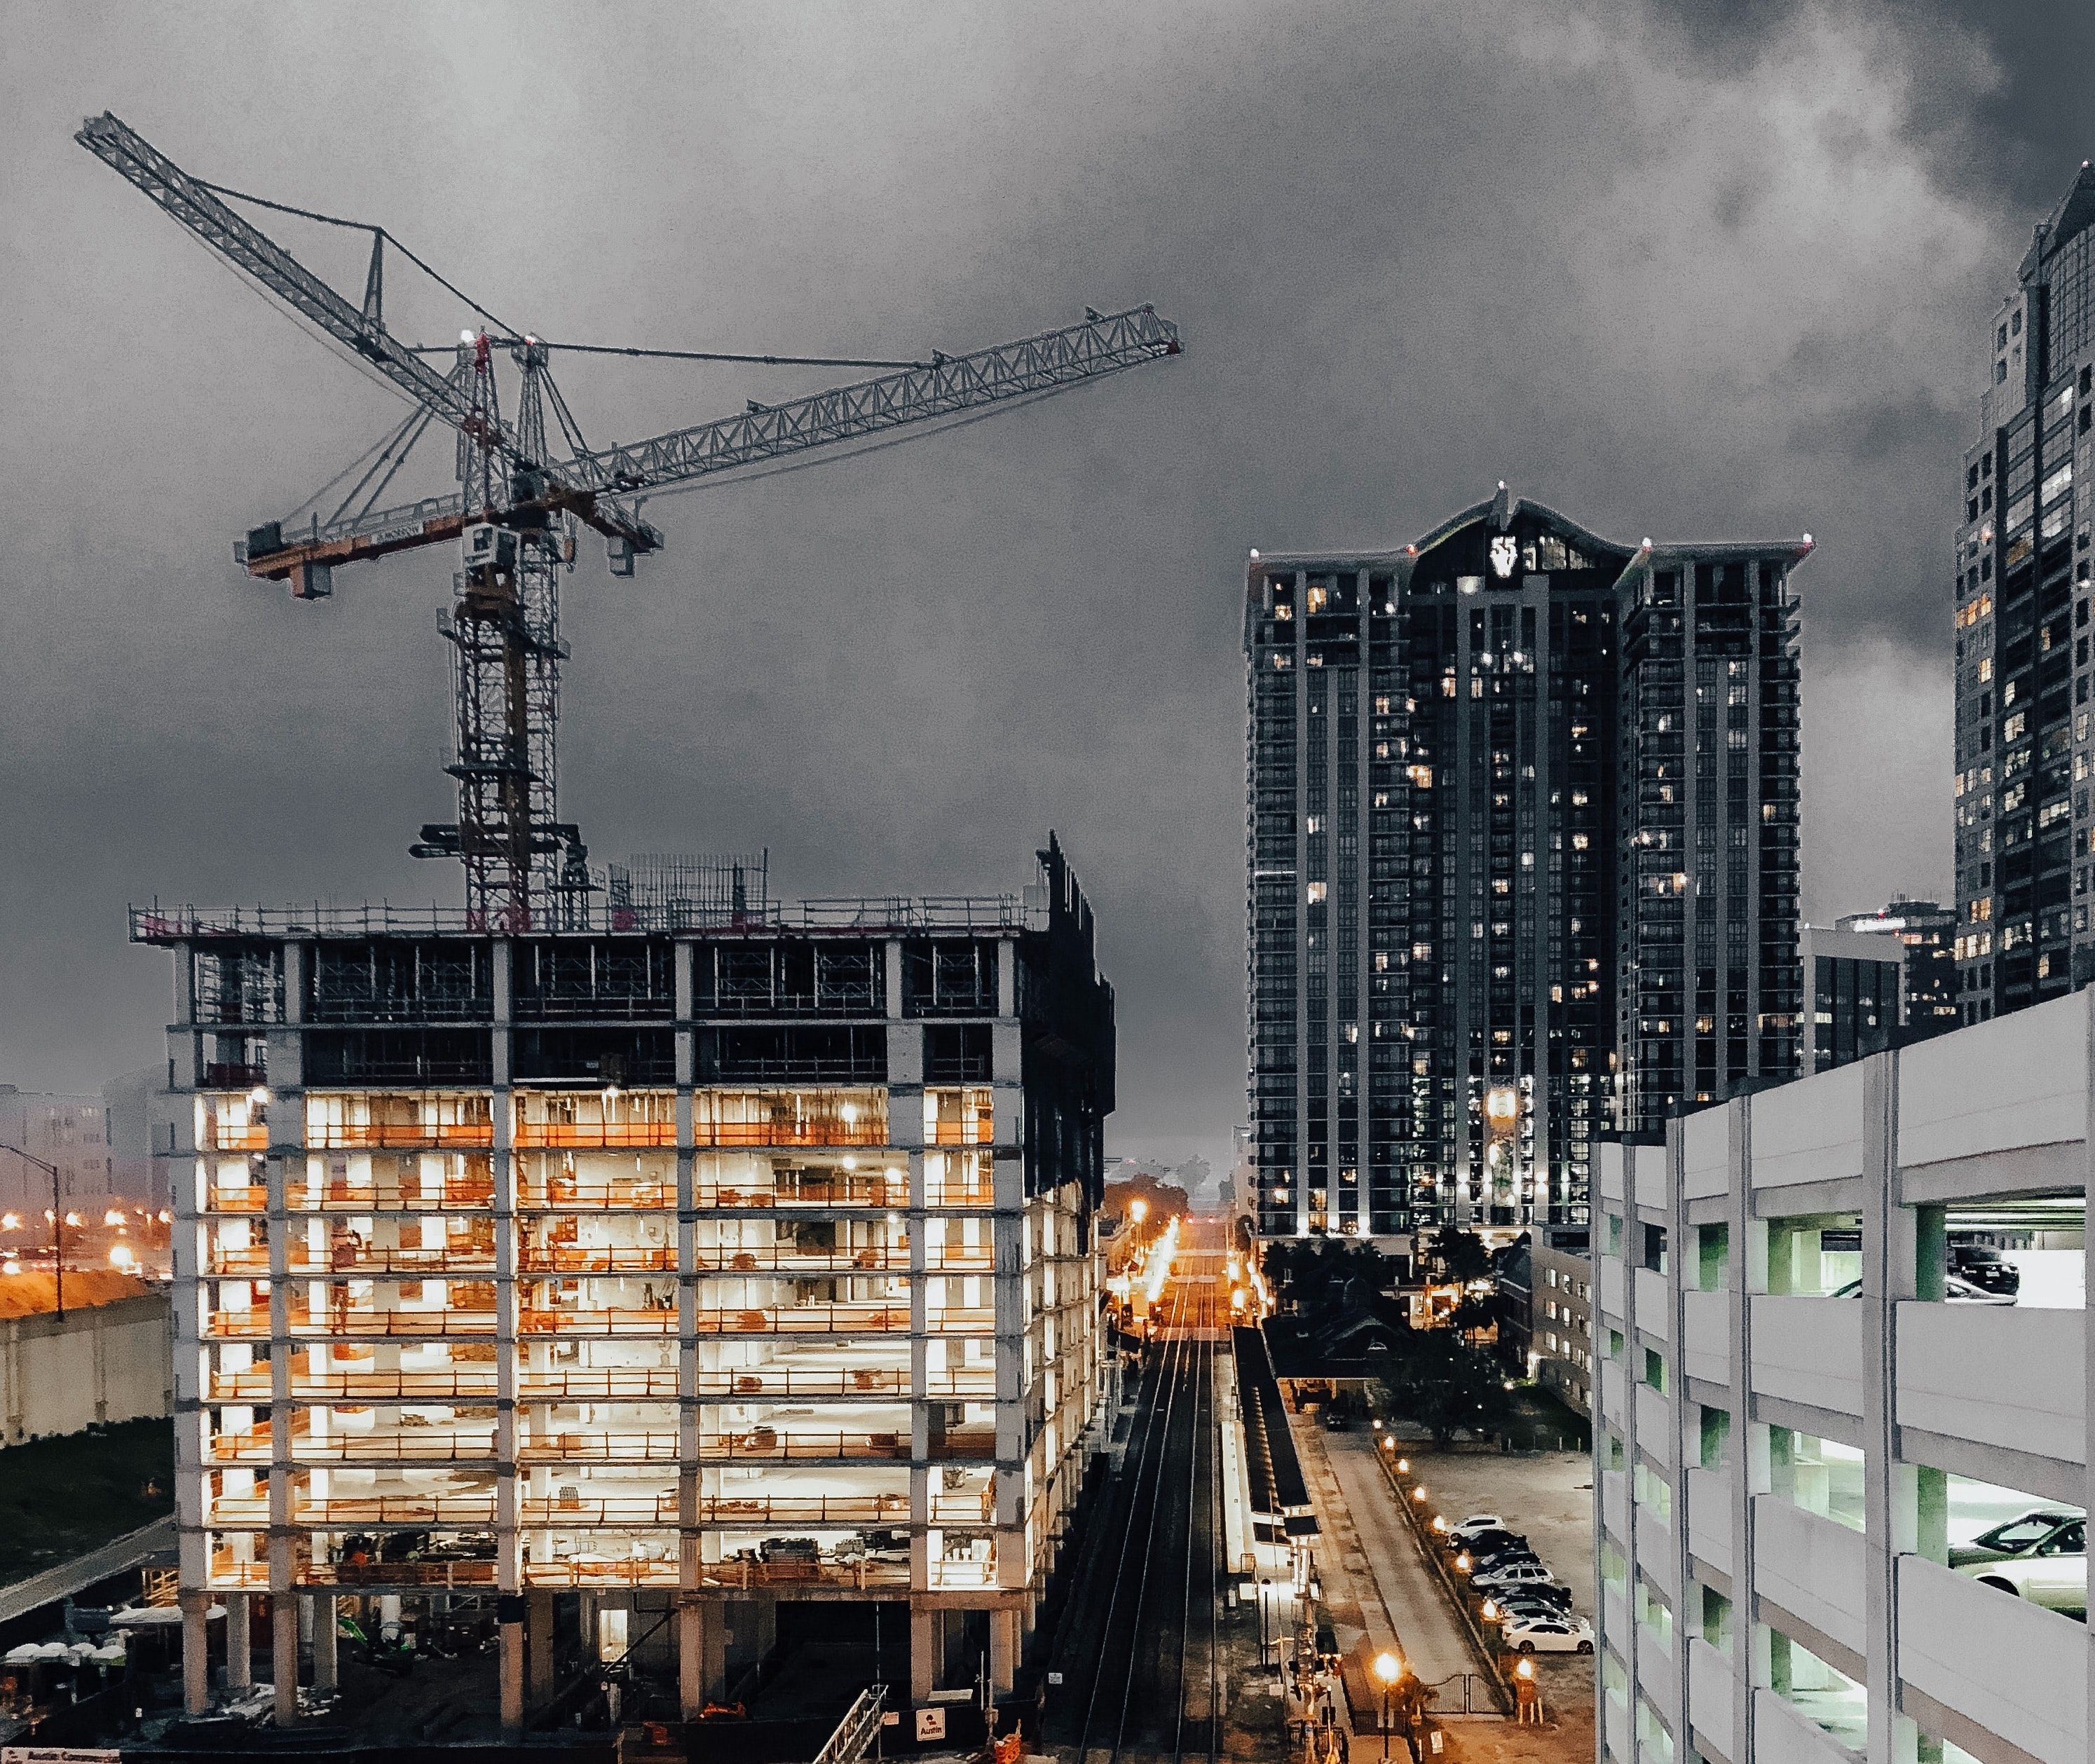
\includegraphics{img/crane.jpg} Photo by Nathan Waters on Unsplash

\end{footnotesize}}

\hypertarget{introduction}{%
\section{Introduction}\label{introduction}}

This is the first in a series of posts offering suggested strategies for
leveraging open source technologies to provide straight-forward
solutions to one of the central challenges in the practice of data
science, i.e.~how to effectively communicate analysis results to clients
and collaborators. The list of open-source technologies (software stack)
we suggest for employment is: linux, R, Shiny, Docker, Git, and Caddy.
In this post we'll make use of two cloud services: Github and Amazon Web
Service (AWS). Further posts will describe alternate constructions,
e.g.~using the low cost cloud service: Hetzner.

Also described in other posts are strategies that avoid Github and
docker-compose. This approach provides a simpler initial construction,
but a more labor intensive updating process.

This initial post provides a minimal, proof-of-concept example of how to
apply these technologies for hosting an interactive Shiny application.

In the following we start with a very simple, but hopefully still
useful, stand-alone Shiny app developed on our local workstation. Then
after some straightforward interfacing with the AWS environment, we push
the Shiny app into the cloud, and end up with a secure (encrypted and
authenticated) app running on a website with a custom domain name.

\hypertarget{methods}{%
\section{Methods}\label{methods}}

Start by creating a repository (repo) for the project. The best way to
do this is to initiate the repo on Github and then \texttt{clone} it to
your local workstation. Start by logging in to Github and creating a new
empty repo, call it power1\_app. On your local workstation navigate to
your Shiny development directory, say \texttt{\textasciitilde{}/prj} and
clone the power1\_app repo from Github:

\begin{tcolorbox}[enhanced jigsaw, colbacktitle=quarto-callout-note-color!10!white, leftrule=.75mm, opacitybacktitle=0.6, toprule=.15mm, arc=.35mm, coltitle=black, left=2mm, bottomrule=.15mm, opacityback=0, bottomtitle=1mm, toptitle=1mm, titlerule=0mm, breakable, title=\textcolor{quarto-callout-note-color}{\faInfo}\hspace{0.5em}{Details for creating a Github repo follow:}, colback=white, colframe=quarto-callout-note-color-frame, rightrule=.15mm]

\begin{marginfigure}

{\centering 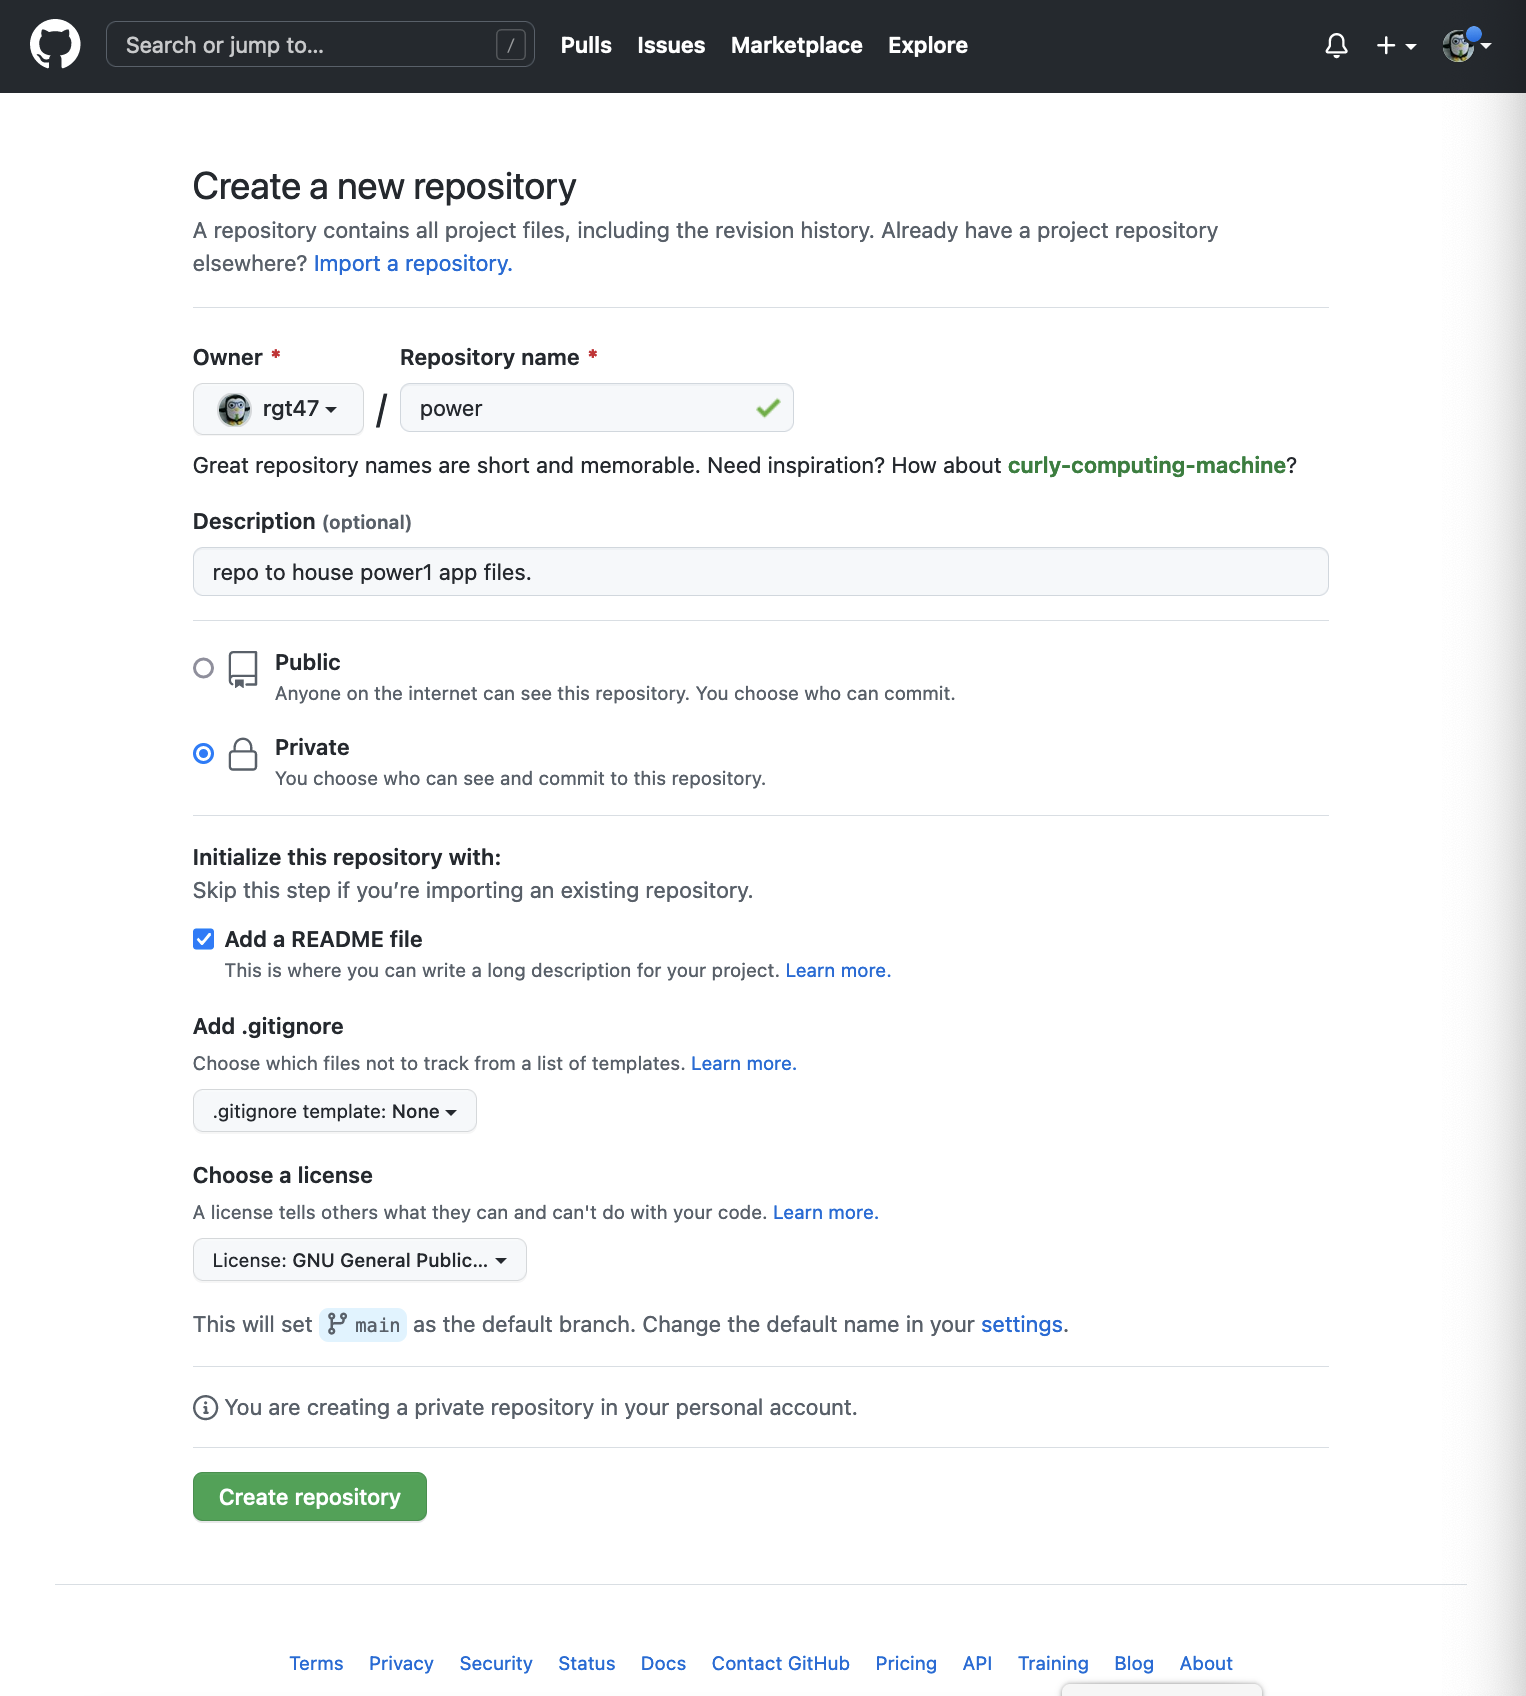
\includegraphics{img/git1.png}

}

\end{marginfigure}

\begin{itemize}
\item
  login to github (screenshot)
\item
  click on \texttt{new}. Then in \texttt{repository\ name} field enter
  \texttt{power1}. (Make the
\item
  make the repo private, we only want to share with our client at this
  point).
\item
  create the repo. Click \texttt{Create\ repository} green button at the
  bottom of the page.
\item
  on your laptop cd to development directory, say \textasciitilde/prj
  and clone the github repo:
\end{itemize}

\begin{Shaded}
\begin{Highlighting}[]
\FunctionTok{git}\NormalTok{ clone https://github.com/rgt47/power1\_app.git}
\end{Highlighting}
\end{Shaded}

\end{tcolorbox}

After cloning the repo to \textasciitilde/prj/power1\_app cd into the
directory and create two new sub-directories, \texttt{power1\_shiny} and
\texttt{site}. These directories will house our shiny app and our web
site landing page file, respectively.

Lets jump ahead to the point where you've just finished developing a new
Shiny app, named \texttt{power1\_shiny} . (The methods described here
apply generically to any Shiny app, but we'll use one of our own for
illustration). See the \texttt{R/Shiny} code for our
\texttt{power1\_shiny} app (\texttt{app.R})
\protect\hyperlink{appendix-1}{here} in appendix 1.

\begin{Shaded}
\begin{Highlighting}[]
\NormalTok{ui }\OtherTok{\textless{}{-}} \FunctionTok{fluidPage}\NormalTok{(}
\FunctionTok{titlePanel}\NormalTok{(}\StringTok{"Power Calculator for Two Group Parallel Designs"}\NormalTok{),}
\FunctionTok{sliderInput}\NormalTok{(}\StringTok{"N"}\NormalTok{, }\StringTok{"Total Sample Size:"}\NormalTok{, }\AttributeTok{min =} \DecValTok{0}\NormalTok{, }\AttributeTok{max =} \DecValTok{300}\NormalTok{, }\AttributeTok{value =} \DecValTok{100}\NormalTok{),}
\FunctionTok{plotOutput}\NormalTok{(}\StringTok{"plot"}\NormalTok{),}
\FunctionTok{verbatimTextOutput}\NormalTok{(}\StringTok{"eff"}\NormalTok{))}

\NormalTok{server }\OtherTok{\textless{}{-}} \ControlFlowTok{function}\NormalTok{(input, output, session) \{}
\NormalTok{  delta }\OtherTok{=} \FunctionTok{seq}\NormalTok{(}\DecValTok{0}\NormalTok{, }\FloatTok{1.5}\NormalTok{,.}\DecValTok{05}\NormalTok{)}
\NormalTok{  pow }\OtherTok{=} \FunctionTok{reactive}\NormalTok{(}\FunctionTok{sapply}\NormalTok{(delta, }\ControlFlowTok{function}\NormalTok{(x) }\FunctionTok{power.t.test}\NormalTok{(input}\SpecialCharTok{$}\NormalTok{N, }\AttributeTok{d=}\NormalTok{x)}\SpecialCharTok{$}\NormalTok{power ))}
\NormalTok{  eff }\OtherTok{=}  \FunctionTok{renderText}\NormalTok{(}\FunctionTok{power.t.test}\NormalTok{(input}\SpecialCharTok{$}\NormalTok{N, }\AttributeTok{power=}\NormalTok{.}\DecValTok{8}\NormalTok{)}\SpecialCharTok{$}\NormalTok{d)}
\NormalTok{  output}\SpecialCharTok{$}\NormalTok{plot }\OtherTok{\textless{}{-}} \FunctionTok{renderPlot}\NormalTok{(\{}
  \FunctionTok{plot}\NormalTok{(delta, }\FunctionTok{pow}\NormalTok{(), }\AttributeTok{cex=}\FloatTok{1.5}\NormalTok{, }\AttributeTok{ylab=}\StringTok{"power"}\NormalTok{)}
  \FunctionTok{abline}\NormalTok{(}\AttributeTok{h =}\NormalTok{ .}\DecValTok{8}\NormalTok{,  }\AttributeTok{col =} \StringTok{"red"}\NormalTok{, }\AttributeTok{lwd =}\FloatTok{2.5}\NormalTok{, }\AttributeTok{lty =} \DecValTok{4}\NormalTok{)}
  \FunctionTok{abline}\NormalTok{(}\AttributeTok{v =} \FunctionTok{eff}\NormalTok{(), }\AttributeTok{col =} \StringTok{"blue"}\NormalTok{,}\AttributeTok{lwd =}\FloatTok{2.5}\NormalTok{, }\AttributeTok{lty =} \DecValTok{4}\NormalTok{)\})  }
\NormalTok{  output}\SpecialCharTok{$}\NormalTok{eff }\OtherTok{\textless{}{-}} \FunctionTok{renderText}\NormalTok{(}
    \FunctionTok{paste0}\NormalTok{(}\StringTok{"Std. effect detectable with power 80\% = "}\NormalTok{, }\FunctionTok{eff}\NormalTok{()) )}
\NormalTok{\}}
\FunctionTok{shinyApp}\NormalTok{(ui, server)}
\end{Highlighting}
\end{Shaded}

We can test the app locally in our development directory, say
\texttt{power1\_app}, by runnning it with the following command.

\begin{Shaded}
\begin{Highlighting}[]
\ExtensionTok{R} \AttributeTok{{-}e} \StringTok{"library(shiny); runApp(\textquotesingle{}power1\_shiny/app.R\textquotesingle{}, launch=T)"}
\end{Highlighting}
\end{Shaded}

This command will run the R program, load the Shiny package, and launch
the app in your default browser.

Figure 1 below shows the Shiny app running locally in a browser, it
consists of a widget to select the sample size and provide a dynamic
visualization (2D plot) of the power as a function of the standardized
effect size:

\begin{marginfigure}

{\centering 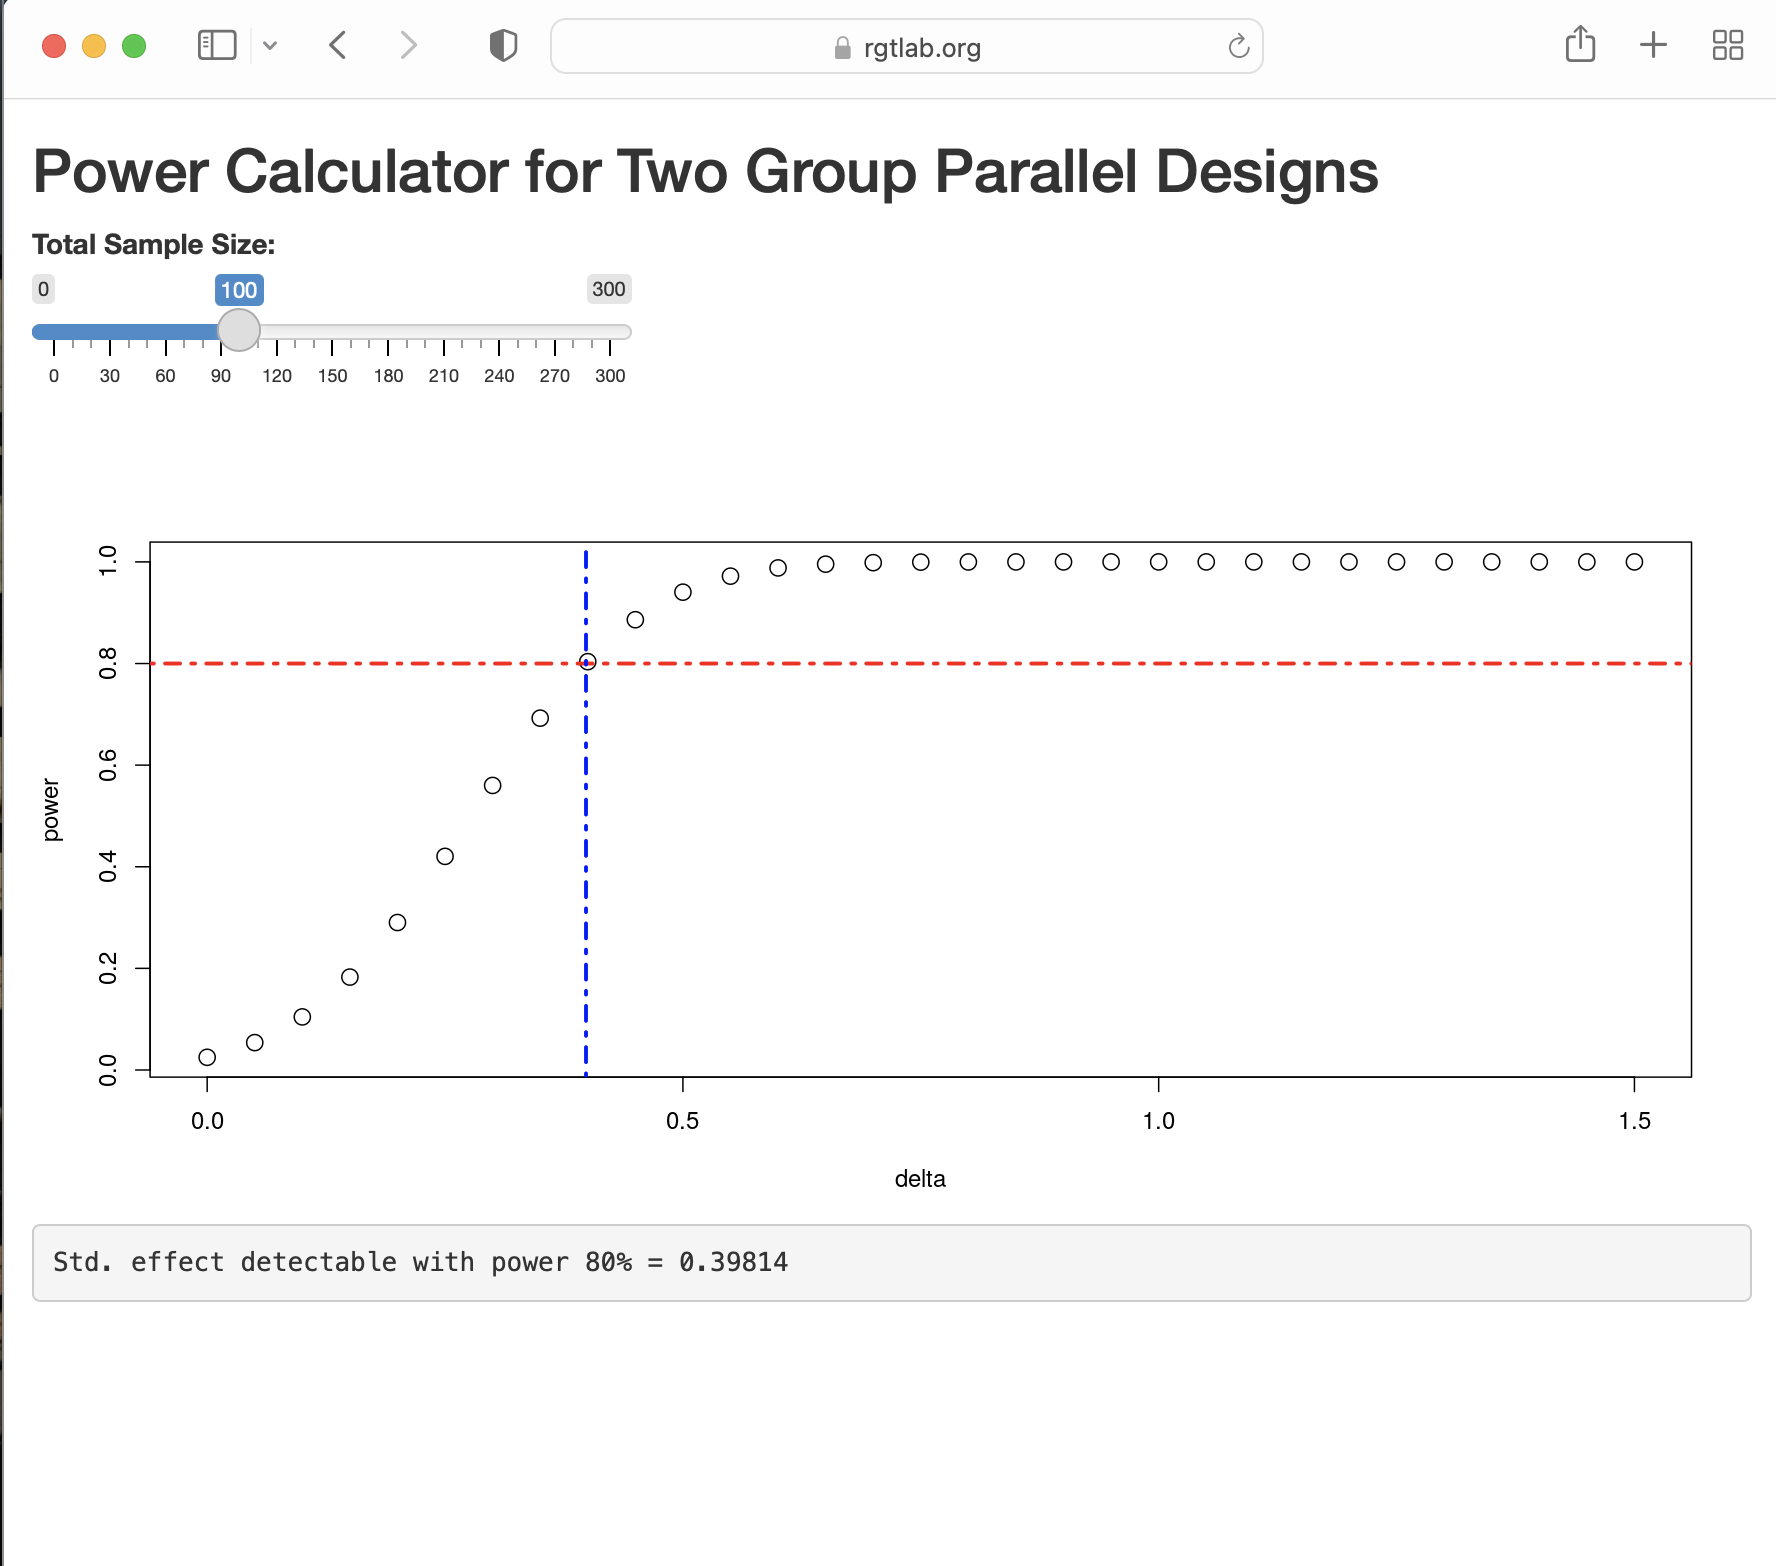
\includegraphics{img/shinyapppower1.png}

}

\caption{\emph{Shiny app}}

\end{marginfigure}

Once we determine our app is working as designed, the next step is to
set up a secure hosting environment on a virtual server. Once the app is
hosted the we simply need to send a link and security credentials to our
collaborators for them to have secure access to the Shiny app. There are
many ways to accomplish the hosting. Here we'll describe a
straightforward and efficient approach using mainstream cloud services
and open source tools. That is, we'll describe how to `spin' up a server
on Amazon Web Service EC2 and in just a few steps, through the
application of Docker, R, Shiny, and Caddy we'll have a fully
functioning secure web app to share with colleagues.

\hypertarget{hosting}{%
\subsection{Hosting}\label{hosting}}

\begin{marginfigure}

{\centering 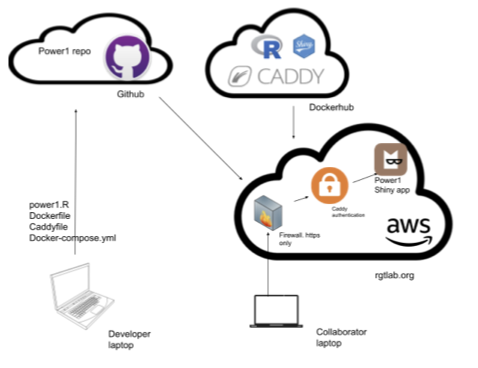
\includegraphics{img/blogdockerizeflow.png}

}

\caption{\emph{Data flow }}

\end{marginfigure}

Figure 2 illustrates the tools we'll use and the flow of program and
configuration files. In order to host \texttt{power1} online we'll need
to complete the following tasks:

\begin{enumerate}
\def\labelenumi{\arabic{enumi}.}
\tightlist
\item
  create a virtual server (connected via ssh) with a firewall
\item
  obtain a static IP address (to identify the server online)
\item
  obtain a domain name (name for IP address)
\item
  install and configure a webserver (tool to interact with https
  protocol requests and respond)
\item
  obtain and install an SSL certificate (to allow encrypted
  communication)
\item
  setup an authentication method (password protection)
\item
  configure a reverse proxy method (translate https, port 443, requests
  to Shiny, port 3838)
\end{enumerate}

At first glance these 7 requirements can appear daunting, but on closer
inspection all can be met with relative ease and minimal cost ( using a
cloud-hosting service, e.g.~Amazon's EC2 or Digital Ocean, and a
``leased'' domain name from, e.g.~GoDaddy, or Amazon's Route 53) or no
cost( if you have your own server with IP address, and domain name)

\hypertarget{select-a-hosting-service}{%
\subsection{Select a hosting service}\label{select-a-hosting-service}}

There are a number of cloud based server options: Microsoft Azure,
Oracle, Google Cloud, Amazon AWS EC2, Digital Ocean to name a few. Each
has their own approach to setting up a custom virtual server. Several
have free or low-cost service tiers available.

An overview of the process with EC2 follows. Detailed instructions for
AWS EC2 are covered in an earlier post
\href{https://focusonr.org/posts/setupaws/}{here}.

\begin{enumerate}
\def\labelenumi{\arabic{enumi}.}
\setcounter{enumi}{-1}
\tightlist
\item
  Create an account or sign in.
\item
  Set up an interactive environment with AWS server.

  \begin{enumerate}
  \def\labelenumii{\alph{enumii}.}
  \tightlist
  \item
    define ssh key-pair.
  \item
    configure firewall.
  \item
    request static IP.
  \item
    obtain domain name.
  \item
    select an instance and launch server.
  \end{enumerate}
\end{enumerate}

Once the server is available connect via ssh, and login,

The only necessary software to install is docker and git. Install both
with the following commands:

\begin{Shaded}
\begin{Highlighting}[]
\FunctionTok{sudo}\NormalTok{ apt install }\AttributeTok{{-}y}\NormalTok{ git}
\FunctionTok{sudo}\NormalTok{ snap install docker.io}
\end{Highlighting}
\end{Shaded}

Once the host is set up and the requisite software installed we'll have
a customized virtual server wtih a static IP address, and a unique
domain name and firewall in place. In other words, items 1, 2, and 3
from our \texttt{hosting} list above will be taken care of.

\hypertarget{website}{%
\subsection{Website}\label{website}}

To configure the web server and containerize our app we need to add
three files to the repo, to go along with our Shiny app.

We'll use a slightly indirect route to create and place the necessary
files on the server but this approach will allow to do all our
countinuing development on our local workstation and have the web app be
automatically continually undated. We'll create the configuration files
we need on our workstation and push them github and from there they can
be accessed from our server.

These three configuation files are:

\begin{enumerate}
\def\labelenumi{\arabic{enumi}.}
\tightlist
\item
  a Docker configuration file (default name \texttt{Dockerfile})
\end{enumerate}

\marginnote{\begin{footnotesize}

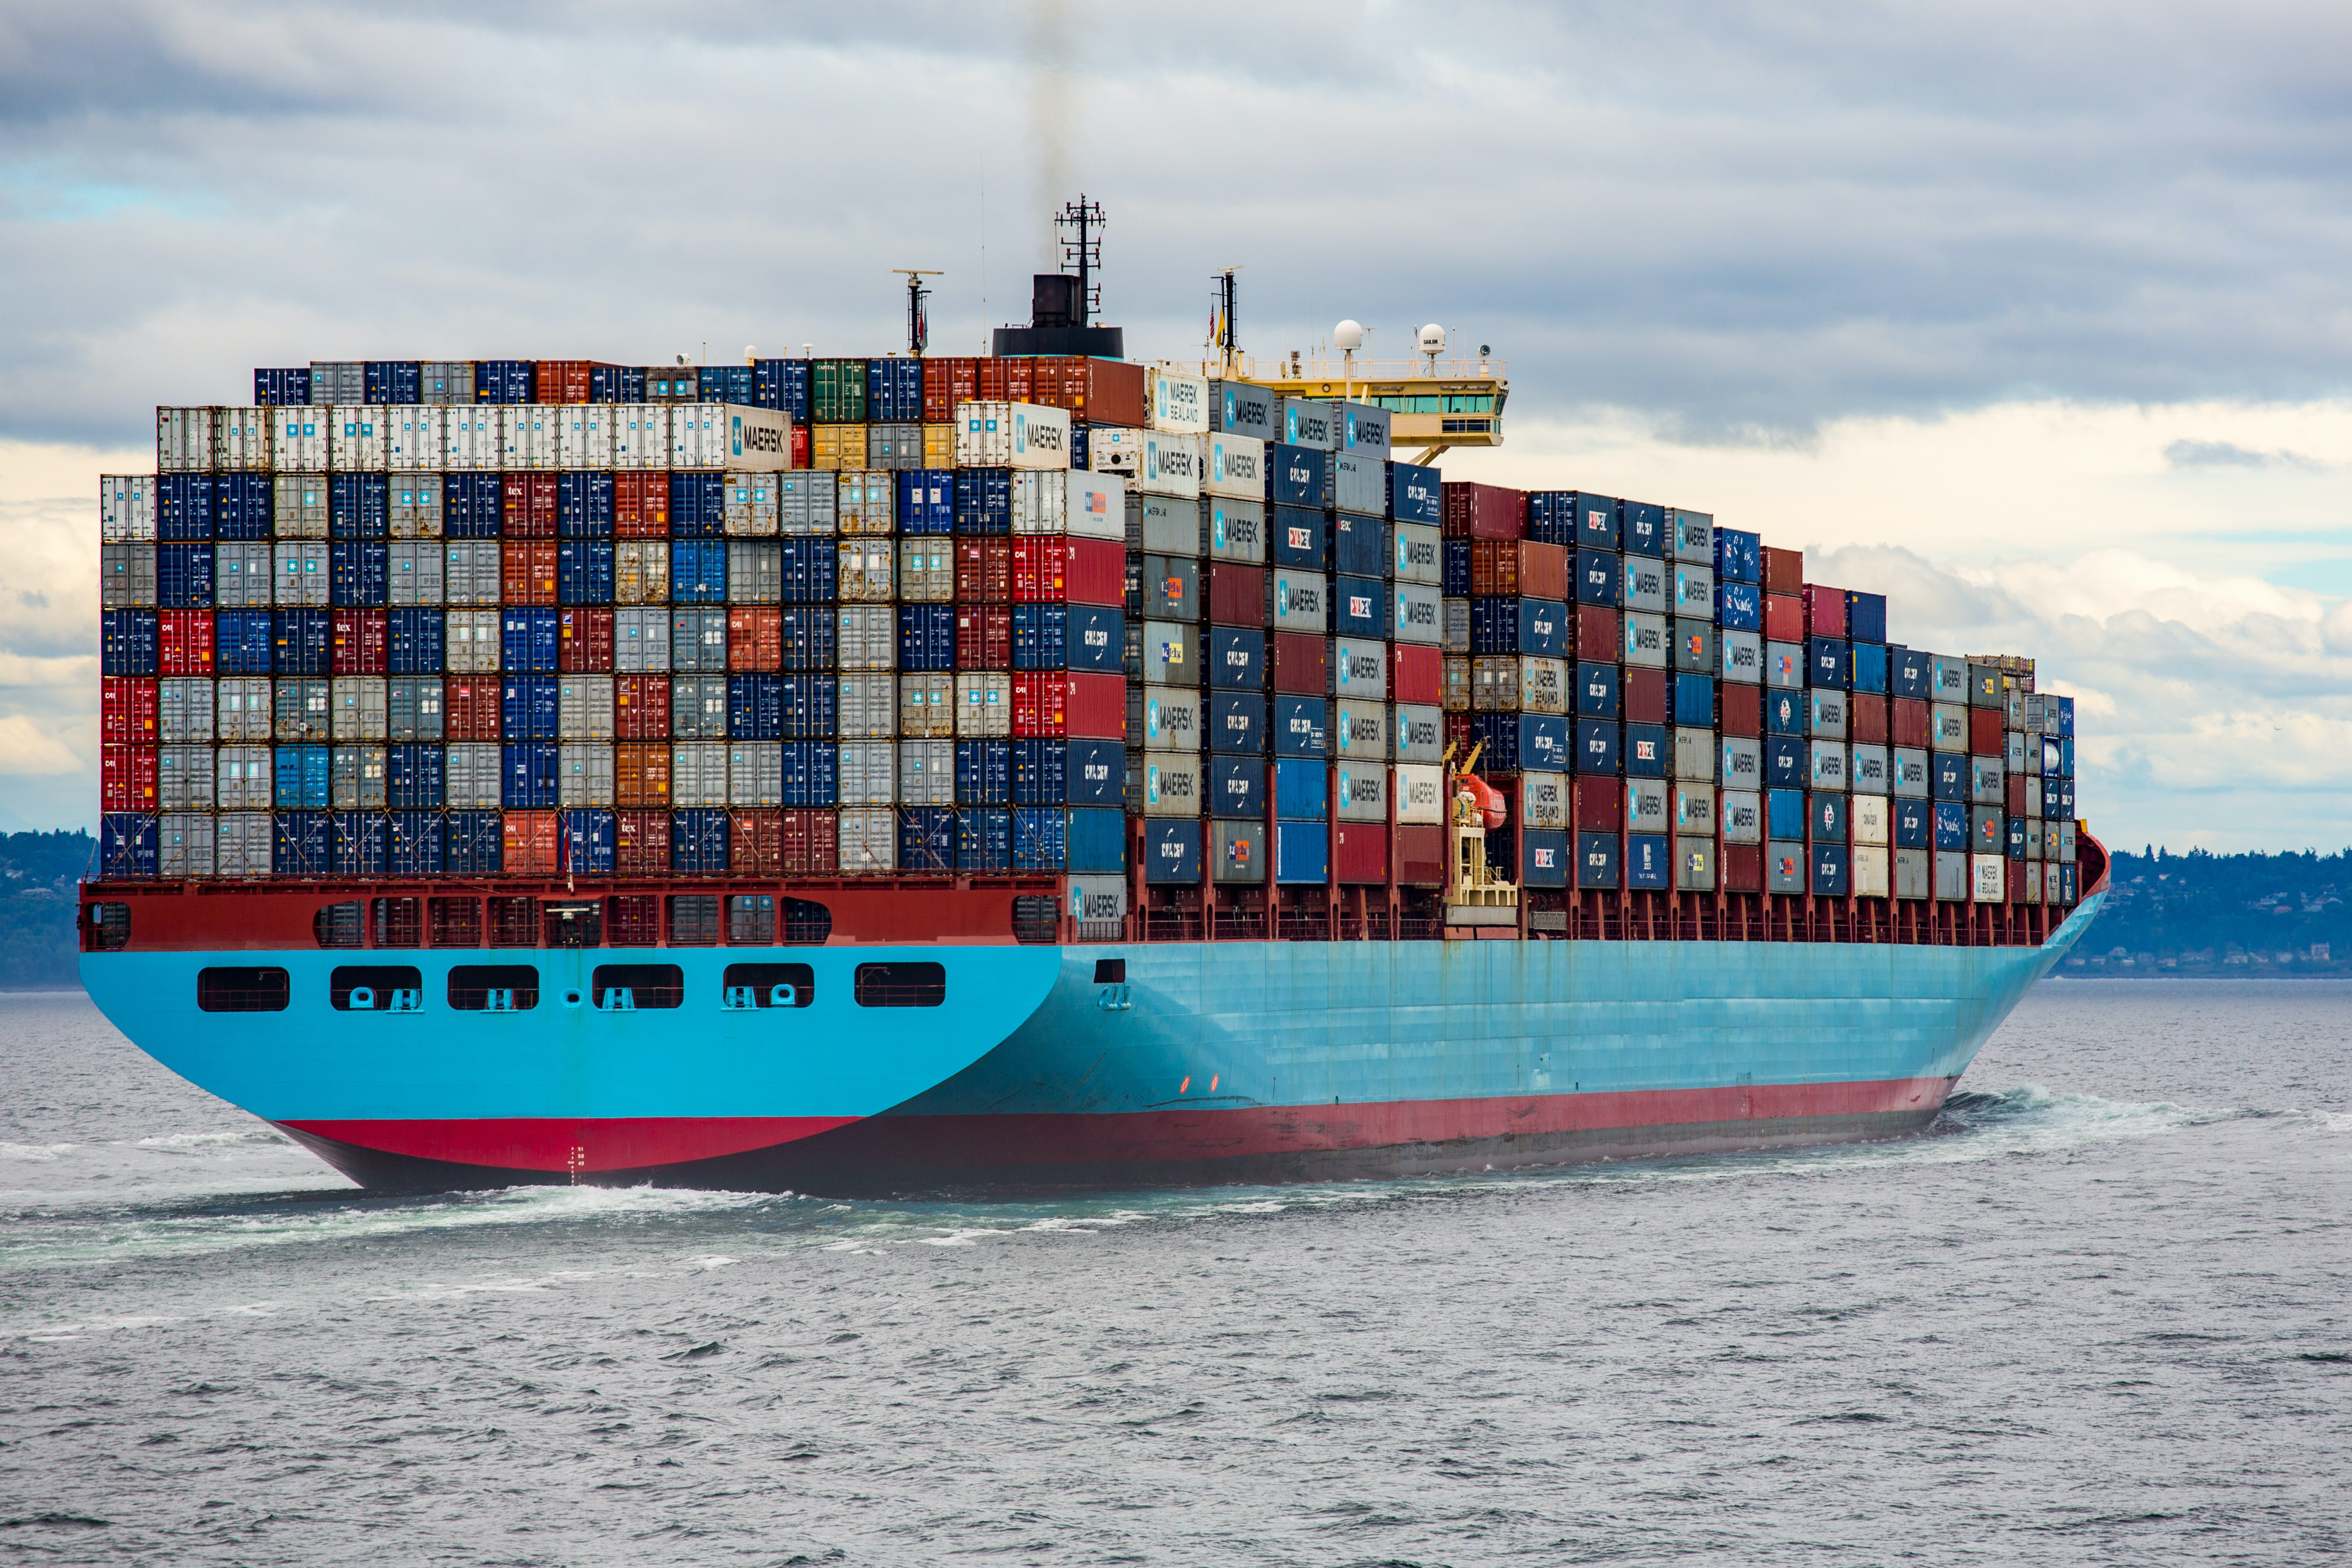
\includegraphics{img/docker1.jpg} Photo by Ian Taylor on Unsplash

\end{footnotesize}}

We'll use docker to access R/Shiny, and docker-compose to access Caddy,
our webserver. The first file is the dockerfile. Here is our minimal
dockerfile with comments:

\begin{Shaded}
\begin{Highlighting}[]
\NormalTok{from rocker}\SpecialCharTok{/}\NormalTok{shiny}\SpecialCharTok{:}\DecValTok{4}\NormalTok{.}\FloatTok{2.0}
\NormalTok{copy }\SpecialCharTok{/}\NormalTok{power1\_shiny}\SpecialCharTok{/}\ErrorTok{*} \ErrorTok{/}\NormalTok{srv}\SpecialCharTok{/}\NormalTok{shiny}\SpecialCharTok{{-}}\NormalTok{server}\SpecialCharTok{/}
\NormalTok{cmd [}\StringTok{"/usr/bin/shiny{-}server"}\NormalTok{]}
\end{Highlighting}
\end{Shaded}

\begin{enumerate}
\def\labelenumi{\arabic{enumi}.}
\tightlist
\item
  Grab the latest rocker/Shiny image from Docker Hub to use as a base
  image.
\item
  Copy the Shiny code to the default location for shiny-server
\item
  Run the Shiny-server using the default app code
\end{enumerate}

This configuration file instructs Docker to build a container based on a
Rocker/Shiny image (which itself is a ubuntu image with R and Shiny
installed) then copy into the container the \texttt{power1\_shiny.R}
code and finally launch Shiny on (default) port 3838. We placed the
power1\_app.R code in the default location \texttt{/srv/shiny-server} we
only need to start the server and it will find the shiny program.

\begin{enumerate}
\def\labelenumi{\arabic{enumi}.}
\setcounter{enumi}{1}
\tightlist
\item
  a Caddy web server configuration file (default name
  \texttt{Caddyfile})
\end{enumerate}

We'll use \texttt{Caddy} as our web server. Caddy is an open-source tool
that has the very useful feature of automating the acquiring and
installing of an SSL certificate. An SSL cert is required by most
browsers to use the encrypted communication protocol https.

Caddy is configured with a file named \texttt{Caddyfile}. We use the
caddy configuration file to specify three critical things.

\begin{enumerate}
\def\labelenumi{\arabic{enumi}.}
\tightlist
\item
  the site domain name.
\item
  the `reverse proxy' map that redirects requests to port 443 (ssl port)
  to port 3838 (Shiny port).
\item
  add login credentials for bob/vanilla47:
\end{enumerate}

Our barebones Caddyfile looks like this:

\begin{Shaded}
\begin{Highlighting}[]
\CommentTok{\# use caddy auth tool to generate a password via the \textasciigrave{}bcrypt\textasciigrave{} algorithm. }
\CommentTok{\# \textgreater{} caddy hash{-}password {-}{-}plaintext vanilla47 }
\NormalTok{rgtlab.org \{}
\NormalTok{    basicauth }\SpecialCharTok{*} \ErrorTok{/}\NormalTok{power1\_shiny}\SpecialCharTok{/}\ErrorTok{*}\NormalTok{ \{}
\NormalTok{        bob }\SpecialCharTok{$}\NormalTok{2a}\SpecialCharTok{$}\DecValTok{14}\SpecialCharTok{$}\NormalTok{pYWd5O7JqNeGLS4m4CKkzemM2pq5ezn9bcTDowofZTl5wRVl8NTJm}
\NormalTok{    \}}
\NormalTok{    root }\SpecialCharTok{*} \ErrorTok{/}\NormalTok{srv}
\NormalTok{    handle\_path }\SpecialCharTok{/}\NormalTok{power1\_shiny}\SpecialCharTok{/}\ErrorTok{*}\NormalTok{ \{}
\NormalTok{            reverse\_proxy power1\_shiny}\SpecialCharTok{:}\DecValTok{3838}
\NormalTok{    \}}
\NormalTok{    file\_server}
\NormalTok{\}}

\StringTok{\textasciigrave{}\textasciigrave{}\textasciigrave{}}\AttributeTok{sh}
\AttributeTok{\# use caddy auth tool to generate a password via the }\StringTok{\textasciigrave{}}\NormalTok{bcrypt}\StringTok{\textasciigrave{}}\AttributeTok{ algorithm. }
\AttributeTok{\textgreater{} caddy hash{-}password {-}{-}plaintext vanilla47 }
\AttributeTok{caddy hash{-}password }
\AttributeTok{rgtlab.org \{}
\AttributeTok{basicauth * /power1\_shiny/* \{}
\AttributeTok{        bob $2a$14$pYWd5O7JqNeGLS4m4CKkzemM2pq5ezn9bcTDowofZTl5wRVl8NTJm}
\AttributeTok{    \}}
\AttributeTok{    root * /var/www/html}
\AttributeTok{    handle\_path /power1\_shiny/* \{}
\AttributeTok{            reverse\_proxy 0.0.0.0:3838}
\AttributeTok{    \}}
\AttributeTok{    file\_server}
\AttributeTok{\}}
\end{Highlighting}
\end{Shaded}

\begin{verbatim}

We can accomplish what we need for items 4, 5, and 7 through the
Caddyfile.

Note:

-   rgtlab.org is our domain name
-   `handle_path` maps all https requests to port 3838 where Shiny is
    listening.

Providing our servers domain name, `rgtlab.org` is sufficient to
initiate an exchange with the `letsencrypt` service to generates an SSL certificate.

And a third file is the docker compose file that containerizes our
Shiny app, pulls a caddy webserver image from Docker Hub and creates a
local network for the two containers to communicate in.

3.   a Docker-compose configuration file (default name
    `docker-compose.yml`).

The docker-compose.yml file:


```{.r .cell-code  code-fold="true" code-summary="`docker-compose.yml`. Show the code"}
version: "3.7"

services:
  power1_shiny:
    build: .
    expose:
    - "3838"
  caddy:
    image: caddy:2.3.0-alpine
    ports:
      - "80:80"
      - "443:443"
    volumes:
      - $PWD/Caddyfile:/etc/caddy/Caddyfile
      - $PWD/site:/srv
      - caddy_data:/data
volumes:
    caddy_data:
\end{verbatim}

Lastly, we need an html file, \texttt{index.html} that provides the
landing page for our server.

\begin{Shaded}
\begin{Highlighting}[]
\SpecialCharTok{\textless{}!}\NormalTok{DOCTYPE html}\SpecialCharTok{\textgreater{}}
\ErrorTok{\textless{}}\NormalTok{html}\SpecialCharTok{\textgreater{}}
  \ErrorTok{\textless{}}\NormalTok{body}\SpecialCharTok{\textgreater{}}
    \ErrorTok{\textless{}}\NormalTok{h1}\SpecialCharTok{\textgreater{}}\NormalTok{Power1 app}\SpecialCharTok{\textless{}}\ErrorTok{/}\NormalTok{h1}\SpecialCharTok{\textgreater{}}
    \ErrorTok{\textless{}}\NormalTok{ul}\SpecialCharTok{\textgreater{}}
      \ErrorTok{\textless{}}\NormalTok{li}\SpecialCharTok{\textgreater{}}\ErrorTok{\textless{}}\NormalTok{a href}\OtherTok{=}\StringTok{"./power1\_shiny/"}\SpecialCharTok{\textgreater{}}\NormalTok{Power1 app}\SpecialCharTok{\textless{}}\ErrorTok{/}\NormalTok{a}\SpecialCharTok{\textgreater{}}\ErrorTok{\textless{}/}\NormalTok{li}\SpecialCharTok{\textgreater{}}
    \ErrorTok{\textless{}/}\NormalTok{ul}\SpecialCharTok{\textgreater{}}
  \ErrorTok{\textless{}/}\NormalTok{body}\SpecialCharTok{\textgreater{}}
\ErrorTok{\textless{}/}\NormalTok{html}\SpecialCharTok{\textgreater{}} 
\end{Highlighting}
\end{Shaded}

At this point our \texttt{power1\_app} repo looks like this:

\begin{Shaded}
\begin{Highlighting}[]
\NormalTok{.}
\NormalTok{├── Caddyfile}
\NormalTok{├── Dockerfile}
\NormalTok{├── README.md}
\NormalTok{├── docker{-}compose.yml}
\NormalTok{├── power1\_shiny}
\NormalTok{│   └── app.R}
\NormalTok{└── site}
\NormalTok{    └── index.html}
\end{Highlighting}
\end{Shaded}

\hypertarget{github}{%
\section{Github}\label{github}}

Push the new content to Github.

\begin{Shaded}
\begin{Highlighting}[]
\FunctionTok{git}\NormalTok{ push}
\end{Highlighting}
\end{Shaded}

Next login to the virtual server and clone the repo from Github.

\begin{Shaded}
\begin{Highlighting}[]
\FunctionTok{ssh}\NormalTok{ rgtlab.org}
\FunctionTok{git}\NormalTok{ clone https://github.com/rgt47/power1\_app.git}
\end{Highlighting}
\end{Shaded}

Lastly, cd into \texttt{power1\_app} directory and run

\begin{Shaded}
\begin{Highlighting}[]
\ExtensionTok{docker}\NormalTok{ compose up }\AttributeTok{{-}d}
\end{Highlighting}
\end{Shaded}

and you're good to go! The power1\_shiny app is available at

\begin{Shaded}
\begin{Highlighting}[]
\ExtensionTok{https://rgtlab.org/}
\end{Highlighting}
\end{Shaded}

\hypertarget{appendices}{%
\section{Appendices}\label{appendices}}

\hypertarget{appendix-1}{%
\subsection{Appendix-1}\label{appendix-1}}

\hypertarget{app.r}{%
\subsection{App.R}\label{app.r}}

Consider an app that is a balance of simple and functional -- one that
calculates the power for a 2-sample t-test as a function of the
standardized effect size. re is our shiny app \texttt{power1\_shiny.R}:

Consider the power1.R file:

\begin{Shaded}
\begin{Highlighting}[]

\ExtensionTok{ui} \OperatorTok{\textless{}}\NormalTok{{-} fluidPage}\ErrorTok{(}
\ExtensionTok{titlePanel}\ErrorTok{(}\StringTok{"Power Calculator for Two Group Parallel Designs"}\KeywordTok{)}\ExtensionTok{,}
\ExtensionTok{sliderInput}\ErrorTok{(}\StringTok{"N"}\ExtensionTok{,} \StringTok{"Total Sample Size:"}\NormalTok{, min = 0, max = 300, value = 100}\KeywordTok{)}\ExtensionTok{,}
\ExtensionTok{plotOutput}\ErrorTok{(}\StringTok{"plot"}\KeywordTok{)}\ExtensionTok{,}
\ExtensionTok{verbatimTextOutput}\ErrorTok{(}\StringTok{"eff"}\KeywordTok{))}

\ExtensionTok{server} \OperatorTok{\textless{}}\NormalTok{{-} function}\ErrorTok{(}\ExtensionTok{input,}\NormalTok{ output, session}\KeywordTok{)} \KeywordTok{\{}
  \ExtensionTok{delta}\NormalTok{ = seq}\ErrorTok{(}\ExtensionTok{0,}\NormalTok{ 1.5,.05}\KeywordTok{)}
  \ExtensionTok{pow}\NormalTok{ = reactive}\ErrorTok{(}\ExtensionTok{sapply}\ErrorTok{(}\ExtensionTok{delta,}\NormalTok{ function}\ErrorTok{(}\ExtensionTok{x}\KeywordTok{)} \ExtensionTok{power.t.test}\ErrorTok{(}\ExtensionTok{input}\VariableTok{$N}\ExtensionTok{,}\NormalTok{ d=x}\KeywordTok{)}\VariableTok{$power} \KeywordTok{))}
  \ExtensionTok{eff}\NormalTok{ =  renderText}\ErrorTok{(}\ExtensionTok{power.t.test}\ErrorTok{(}\ExtensionTok{input}\VariableTok{$N}\ExtensionTok{,}\NormalTok{ power=.8}\KeywordTok{)}\VariableTok{$d}\KeywordTok{)}
  \ExtensionTok{output}\VariableTok{$plot} \OperatorTok{\textless{}}\NormalTok{{-} renderPlot}\ErrorTok{(}\KeywordTok{\{}
  \ExtensionTok{plot}\ErrorTok{(}\ExtensionTok{delta,}\NormalTok{ pow}\ErrorTok{(}\KeywordTok{)}\ExtensionTok{,}\NormalTok{ cex=1.5, ylab=}\StringTok{"power"}\KeywordTok{)}
  \ExtensionTok{abline}\ErrorTok{(}\ExtensionTok{h}\NormalTok{ = .8,  col = }\StringTok{"red"}\NormalTok{, lwd =2.5, lty = 4}\KeywordTok{)}
  \ExtensionTok{abline}\ErrorTok{(}\ExtensionTok{v}\NormalTok{ = eff}\ErrorTok{(}\KeywordTok{)}\ExtensionTok{,}\NormalTok{ col = }\StringTok{"blue"}\NormalTok{,lwd =2.5, lty = 4}\KeywordTok{)\})}  
  \ExtensionTok{output}\VariableTok{$eff} \OperatorTok{\textless{}}\NormalTok{{-} renderText}\ErrorTok{(}
    \ExtensionTok{paste0}\ErrorTok{(}\StringTok{"Std. effect detectable with power 80\% = "}\ExtensionTok{,}\NormalTok{ eff}\ErrorTok{(}\KeywordTok{))} \KeywordTok{)}
\KeywordTok{\}}
\ExtensionTok{shinyApp}\ErrorTok{(}\ExtensionTok{ui,}\NormalTok{ server}\KeywordTok{)}
\end{Highlighting}
\end{Shaded}

The app is designed to be maximally minimal. Using only base R
functions, with a minimum of reactive widgets and layout commands to
keep it simple while still performing a useful function.

\hypertarget{bonus-add-basic-authentication}{%
\subsection{Bonus: Add basic
authentication}\label{bonus-add-basic-authentication}}

add login credentials for bob/vanilla47 to the Caddyfile:

\begin{Shaded}
\begin{Highlighting}[]
\CommentTok{\# use caddy auth tool to generate a password via the \textasciigrave{}bcrypt\textasciigrave{} algorithm. }
\OperatorTok{\textgreater{}}\NormalTok{ caddy }\ExtensionTok{hash{-}password} \AttributeTok{{-}{-}plaintext}\NormalTok{ vanilla47 }
\ExtensionTok{caddy}\NormalTok{ hash{-}password }
\ExtensionTok{rgtlab.org}\NormalTok{ \{}
\ExtensionTok{basicauth} \PreprocessorTok{*}\NormalTok{ /power1\_shiny/}\PreprocessorTok{*}\NormalTok{ \{}
        \ExtensionTok{bob} \VariableTok{$2}\NormalTok{a}\VariableTok{$1}\NormalTok{4}\VariableTok{$pYWd5O7JqNeGLS4m4CKkzemM2pq5ezn9bcTDowofZTl5wRVl8NTJm}
    \ErrorTok{\}}
    \ExtensionTok{root} \PreprocessorTok{*}\NormalTok{ /var/www/html}
    \ExtensionTok{handle\_path}\NormalTok{ /power1\_shiny/}\PreprocessorTok{*}\NormalTok{ \{}
            \ExtensionTok{reverse\_proxy}\NormalTok{ 0.0.0.0:3838}
    \ErrorTok{\}}
    \ExtensionTok{file\_server}
\ErrorTok{\}}
\end{Highlighting}
\end{Shaded}

\hypertarget{tip-1.-docker-on-m1-macbook.}{%
\subsection{Tip 1. Docker on M1
macbook.}\label{tip-1.-docker-on-m1-macbook.}}

To get docker functioning on M1 Mac desktop

\begin{Shaded}
\begin{Highlighting}[]
\ExtensionTok{docker}\NormalTok{ build }\AttributeTok{{-}t}\NormalTok{ power1\_shiny }\AttributeTok{{-}{-}platform}\NormalTok{ linux/x86\_64 .}
\ExtensionTok{docker}\NormalTok{ run }\AttributeTok{{-}d} \AttributeTok{{-}p}\NormalTok{ 80:3838 }\AttributeTok{{-}{-}platform}\NormalTok{ linux/x86\_64 power1\_shiny}
\end{Highlighting}
\end{Shaded}

\hypertarget{tip-2-add-user-to-docker-group-on-server.}{%
\subsection{Tip 2 add user to docker group on
server.}\label{tip-2-add-user-to-docker-group-on-server.}}

Add ubuntu to the docker group to allow docker to run without sudo.

\begin{Shaded}
\begin{Highlighting}[]
\FunctionTok{sudo}\NormalTok{ usermod }\AttributeTok{{-}aG}\NormalTok{ docker }\VariableTok{$\{USER\}}
\end{Highlighting}
\end{Shaded}

\hypertarget{tip-3-ssh-config-file.}{%
\subsection{Tip 3 ssh config file.}\label{tip-3-ssh-config-file.}}

For convenience, construct a \texttt{config} file in
\texttt{\textasciitilde{}/.ssh} as:

\begin{Shaded}
\begin{Highlighting}[]
\ExtensionTok{Host}\NormalTok{ rgtlab.org}
\ExtensionTok{HostName}\NormalTok{ 13.57.139.31 }\CommentTok{\# static IP}
\ExtensionTok{User}\NormalTok{ ubuntu }\CommentTok{\# default user on ubuntu server}
\ExtensionTok{Port}\NormalTok{ 22  }\CommentTok{\# the default port ssh uses}
\ExtensionTok{IdentityFile}\NormalTok{ \textasciitilde{}/Downloads/power1.rsa}
\end{Highlighting}
\end{Shaded}

then you can ssh into the new server with

\begin{Shaded}
\begin{Highlighting}[]
\FunctionTok{sh}\OperatorTok{\textgreater{}}\NormalTok{ ssh rgtlab.org }
\end{Highlighting}
\end{Shaded}

\hypertarget{references}{%
\section{References}\label{references}}

\begin{itemize}
\tightlist
\item
  \href{https://focusonr.org/posts/setupaws/}{Focus on R: a new qblog -
  Set up a virtual server on AWS (in anticipation of hosting Shiny
  apps)}
\item
  \href{https://hosting.analythium.io/shiny-apps-with-docker-compose-part-1-development/}{Shiny
  Apps with Docker Compose, Part 1: Development}
\item
  \href{https://hosting.analythium.io/shiny-apps-with-docker-compose-part-2-production/}{Shiny
  Apps with Docker Compose, Part 2: Production}
\end{itemize}



\end{document}
